%The modern world is moving towards digitalization at a high pace, which aims to make it smart and interconnected. 
%This transformation comes with the ever-increasing use of connected devices and services, which oftentimes carry sensitive data and are not always protected sufficiently.
%As a result, there is a rising number of cybercrime incidents and subsequent damages estimated to more than \$1 trillion worldwide.

%Compounding on top of the situation is a mismatch between demand and supply of cybersecurity professionals and a public, which is in large parts not aware of the risks posed by the use of connected IT technology.
%Cybercriminals can often easily exploit these unaware people to gain access to restricted systems and data.
%%People who are unaware of potential risks are often a weak spot and can be exploited by cyber criminals to access systems and networks. 
%To combat this problem, there's a need for training cybersecurity professionals, as well as to raise awareness at every level of education and the public.
%As a method for raising awareness, teaching principles of cybersecurity and the methods to apply them, live demonstration and hands-on learning with realistic risk scenarios can be an effective tool. \cite{mariano2024wifi}\cite{Cybersec_Edu}


%\section{Goal}
%The goal of this project is to develop a platform with a flexible and expandable architecture, which can be used for demonstration and practice of Pentesting\footnote{penetration testing, see \cref{ssec:cs_methods}} in cybersecurity education.
%A Raspberry Pi will be used as the main device to create a platform that is portable and easy to use.
%It should be able to reliably set up testing environments for various fields of application, to allow a lecturer to demonstrate cyberattacks and students to practice penetration testing in a realistic environment.
%In recent years, trends like the Internet of Things (IoT) have produced many headless\footnote{without any means for direct interaction} devices, which are often linked to smartphones for user interaction, using Wi-Fi or Bluetooth for communication.
%For this reason, wireless communication security in the form of Wi-Fi technology will be implemented as the first application specific testing environment.
%To teach secure design of web applications, the device should be able to host a server with the OWASP Juice Shop\footnote{is a web security training program, see \cref{ssec:juice_shop}}, which again ties into the security of IoT devices, because they are oftentimes accessed via web interfaces, which are often the source of vulnerabilities \cite[page~174]{Hellmann_2023}.


\begin{frame}[plain]
    \centering
    \LARGE
    \pause
    \textcolor[HTML]{990000}{\textbf{Wie wichtig ist Cybersecurity?}}
\end{frame}

\begin{frame}[plain]
    \centering
    \small
    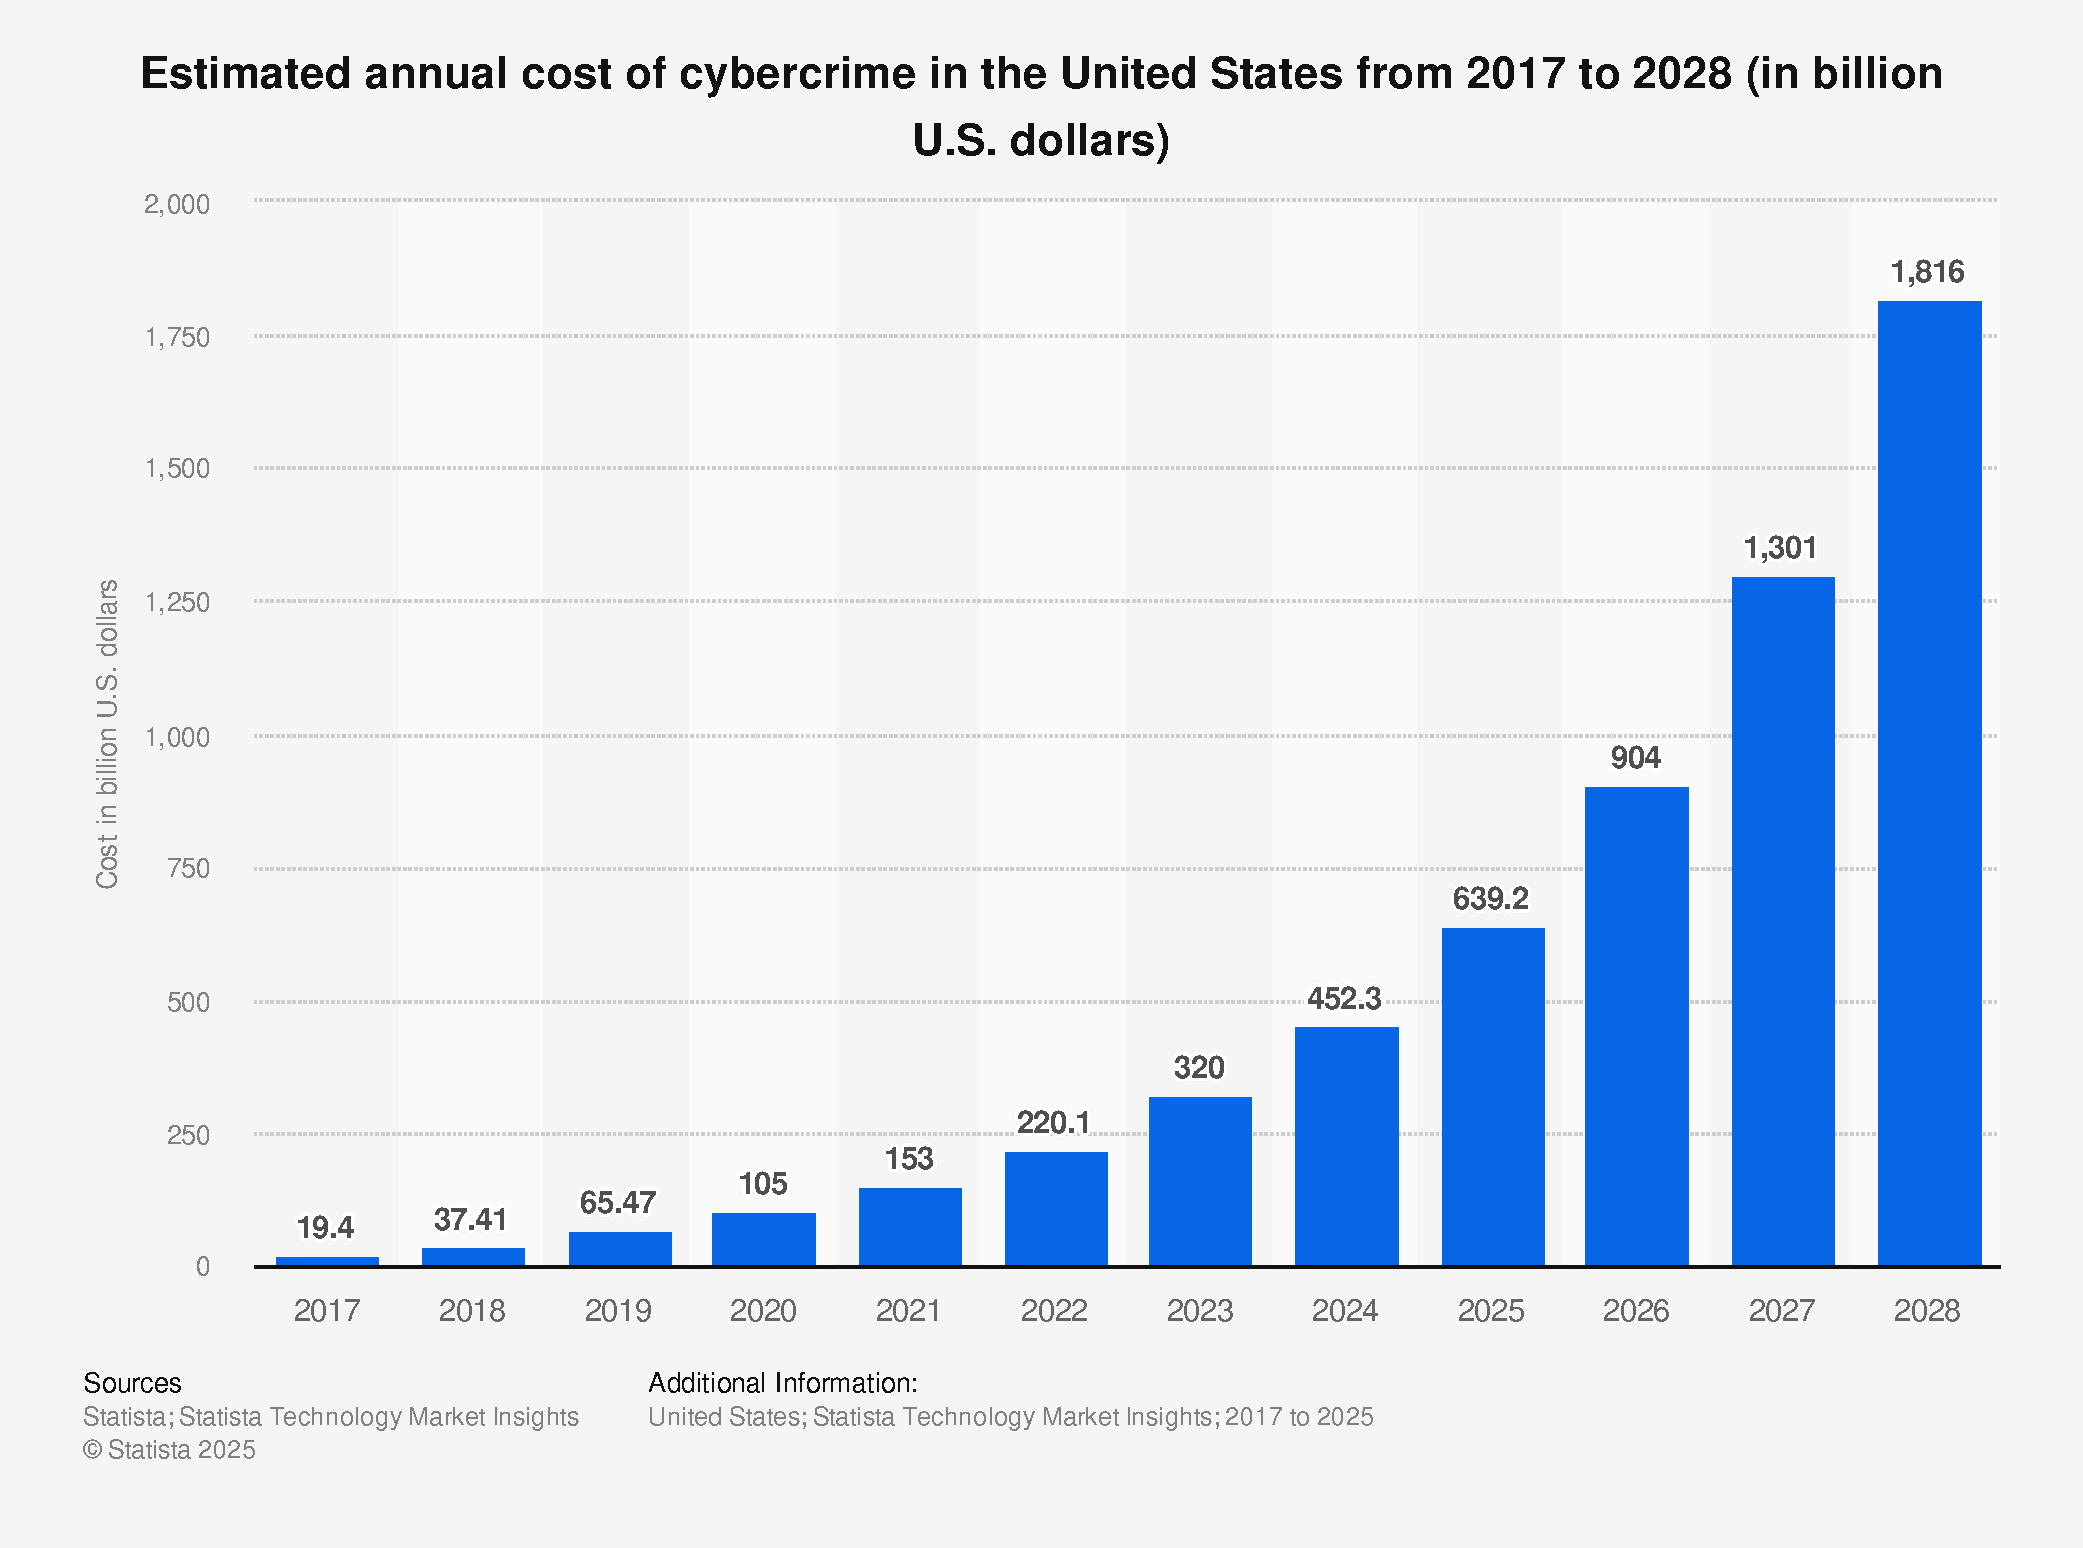
\includegraphics[height=.74\textheight]{figures/statistic_id1399040_annual-cost-of-cybercrime-in-the-us-2017-2028.pdf}
    \vspace{.6cm}
    \\\textbf{"[...] there is a significant mismatch in supply and demand of skilled professionals."}
    \tiny
    \\\textit{Leslie F. Sikos, Paul Haskell-Dowland - Cybersecurity Teaching in Higher Education}
\end{frame}